%TÉCNICA OMNI--------------------
\chapter{TÉCNICA OMNI}
\label{chap:omni}

Neste capítulo será explanada a técnica Omni, mencionada previamente nos capítulos \ref{chap:introducao} e \ref{chap:conceitos}.
A técnica Omni, sua concepção, construção e uso é retirada do trabalho de \cite{Traina2001}.
%TODO Melhorar e expandir

\section{CONCEITOS E DEFINIÇÕES OMNI}
\label{sec:defomni}
Como apresentado anteriormente, as técnicas da família Omni baseiam-se em em uma base de elementos chamada de 
Omni-focos. Estes focos são elementos presentes na base de dados previamente escolhidos, e possuem como função 
servirem de marco para o cálculo das coordenadas Omni de cada elemento presente no banco.

\begin{mydef}
 \label{def:omnifoco}
 Seja um espaço métrico $\mathbb{M} = <\mathbb{S},d>$, uma base de focos Omni é um conjunto 
 $\mathscr{F} = \{f_1, f_2, ..., f_l | f_k \in \mathbb{S}, f_k \neq f_j, l \leq N \}$ onde cada $f_k$ é um foco
 (ou ponto focal) de $\mathbb{S}$, $l$ é o número de focos da base de focos e $N$ é o número de elementos da base de dados.
\end{mydef}

\begin {mydef}
 \label{def:omnicoord}
 Dado um objeto $s_i \in \mathbb{S}$ e a base de focos Omni $\mathscr{F}$, as coordenadas Omni $C_i$ do objeto é o conjunto
 de distâncias de $s_i$ para cada foco em $\mathscr{F}$:
 \begin{equation}
  C_i = \{ <f_k, d(f_k, s_i)>, \forall f_k \in \mathscr{F} \}
 \end{equation}
\end {mydef}

Para distinguir a distância $d(f_k, s_i)$ como uma coordenada, é utilizada a notação $df_k(s_i) = d(f_k, s_i)$.\par
									%TODO Armazenada em uma tabela do banco, indexado por uma B-Tree
Quando um novo objeto é inserido na base de dados, as suas coordenadas Omni são calculadas e armazenadas. Em uma pesquisa por
similaridade, estas coordenadas são utilizadas para podar o número de cálculos de distância, como ilustrado pela figura \ref{fig:rqomni1}.\par

O custo associado a utilização da técnica Omni provém de duas fontes: o tempo para calcular as coordenadas Omni (cálculo da distância
entre o elemento inserido e cada um dos focos) e o espaço físico necessário para armazenar a estrutura Omni, geralmente armazenada em disco.
Como o número de focos necessários usualmente é baixo, estes custos atrelados a técnica Omni são menores do que o ganho
de performance nas consultas.

\section{USO DA BASE DE FOCOS}
Os problemas entre a escolha da base de focos $\mathscr{F}$ e a sua cardinalidade $l$ são intimamente relacionados. Quanto
mais focos, mais espaço e tempo para processamento é necessário. Por isso, é necessário maximizar o ganho de performance com
a menor quantidade possível de focos.

\begin{mydef}
 Dado uma base de focos Omni $\mathscr{F} = \{f_1, f_2, ..., f_l\}$ e uma coleção de objetos $A = \{x_1,x_2,...,x_n\} \subset \mathbb{S}$, a
 região Omni de delimitação mínima (\textit{minimum bounding Omni region - mbOr}) de $A$ é definido como a interseção
 dos intervalos métricos $R_A = |\  ^{l}_{1}I_i$, onde $I_i = [min(d(x_j, f_i)), max(d(x_j, f_i))],\ 1\leq i \leq l,\ 1 \leq j \leq n$. 
\end{mydef}

A ideia gráfica de uma mbOr foi previamente apresentada na figura \ref{fig:rqomni1} para o caso de uma consulta utilizando um único foco.
É possível ver que a mbOr sempre inclui todos os elementos do conjunto-resposta, mas pode incluir elementos que não são pertinentes
ao conjunto-resposta (alarmes falsos). Embora seja necessária mais uma etapa de cálculo de distâncias, o número de cálculos é
reduzido drasticamente com o uso da mbOr.\par

Uma mbOr pode ser reduzida ainda mais com o uso de múltiplos focos, como ilustra a figura \ref{fig:rqomni2}.

\begin{figure}[H]
\centering
\caption{Consulta por abrangência pela técnica Omni utilizando dois focos}
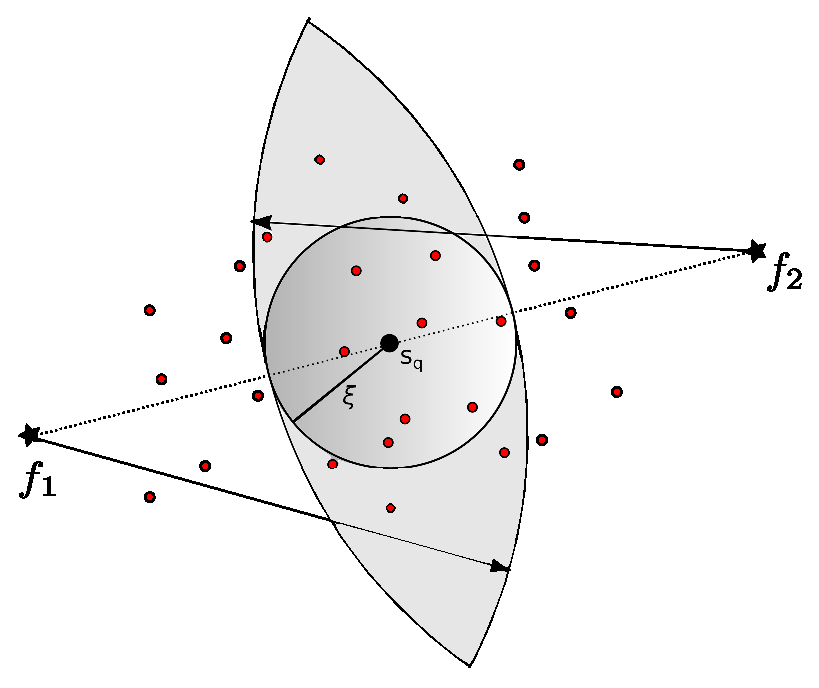
\includegraphics[width=.4\textwidth]{dados/figuras/rg_omni_2.eps}
\fonte{Autoria Própria}
\label{fig:rqomni2}
\end{figure}
								%TODO Arrumar; D + 1
Considerando a família Minkowski de distâncias (métricas $L_p$), um número de focos correspondente ao dobro da
dimensão intrínseca da base de dados seria o suficiente para maximizar a performance da técnica Omni. O uso de mais focos do que o dobro
da dimensão intrínseca do banco traria pouca ou nenhuma redução à mbOr.

\section{ESCOLHA DOS FOCOS}

Para a escolha dos focos Omni, o elemento candidato a foco deve pertencer a base de dados. Isso se deve ao fato de que algumas vezes
é impossível sintetizar um objeto de uma base de dados, como uma impressão digital. O algoritmo utilizado para o encontro dos focos
é o algoritmo HF. Esse algoritmo procura aleatoriamente um elemento $s_1$, encontra o elemento $f_1$ mais distante daquele e o seleciona como
o primeiro foco. Após isso, procura pelo elemento $f_2$ mais longe de $f_1$ e o seleciona como o segundo foco, e armazenando
a distância entre eles como $borda$.\par

O próximo foco é o elemento com as distâncias mais similares aos outros focos previamente escolhidos. Para cada objeto
$s_i$ não escolhido como foco ainda, o erro da distância em relação à borda é:
\begin{equation}
 erro_i = \sum_{k}^{k é foco} |borda - d(f_k, s_i)|
\end{equation}

\begin{algorithm}
\label{alg:hf}
    \caption{Algoritmo HF}
    \KwIn{a base de dados $\mathbb{S}$ e o número de focos $l$}
    \KwOut{base de focos Omni $\mathscr{F}$}
    Início\\
       1.Selecione aleatoriamente um objeto $s_i \in \mathbb{S}$.\\
       2.Encontre o objeto $f_1$ mais longe de $s_i$. Insira $f_1$ em $\mathscr{F}$.\\
       3.Encontre o objeto $f_2$ mais longe de $f_1$. Insira $f_2$ em $\mathscr{F}$.\\
       4.Defina $borda=d(f_1,f_2)$, usada para calcular $erro_i$.\\
      \While{existirem focos a serem determinados}{
	  5.Para cada $s_i \in \mathbb{S},\ s_i \notin \mathscr{F}$: calcule $erro_i$.\\
	  6.Selecione $s_i \in \mathbb{S}$ de tal modo que $erro_i$ seja mínimo.\\
	  7.Insira $s_i$ em $\mathscr{F}$.
      }
\end{algorithm}

O algoritmo HF requer $l*N$ cálculos de distância. O algoritmo \ref{alg:hf} mostra que as etapas 3 e 5 são cálculos
necessários para a determinação das coordenadas Omni de cada objeto. Isso mostra que o algoritmo HF também prepara as
coordenadas Omni da base de dados. Outro fato importante é o da base de focos Omni ser invariável a operações de inserção
ou remoção na base.

%TODO Omni-Seq? OmniB-Tree? OmniR-Tree?
%TODO Citar as outras estruturas, expandir a OmniB-Forest